\documentclass[]{article}
\usepackage{lmodern}
\usepackage{amssymb,amsmath}
\usepackage{ifxetex,ifluatex}
\usepackage{fixltx2e} % provides \textsubscript
\ifnum 0\ifxetex 1\fi\ifluatex 1\fi=0 % if pdftex
  \usepackage[T1]{fontenc}
  \usepackage[utf8]{inputenc}
\else % if luatex or xelatex
  \ifxetex
    \usepackage{mathspec}
  \else
    \usepackage{fontspec}
  \fi
  \defaultfontfeatures{Ligatures=TeX,Scale=MatchLowercase}
\fi
% use upquote if available, for straight quotes in verbatim environments
\IfFileExists{upquote.sty}{\usepackage{upquote}}{}
% use microtype if available
\IfFileExists{microtype.sty}{%
\usepackage{microtype}
\UseMicrotypeSet[protrusion]{basicmath} % disable protrusion for tt fonts
}{}
\usepackage[margin=1in]{geometry}
\usepackage{hyperref}
\hypersetup{unicode=true,
            pdftitle={0\_EDM\_Vis\_Raw},
            pdfauthor={Kurt Ingeman},
            pdfborder={0 0 0},
            breaklinks=true}
\urlstyle{same}  % don't use monospace font for urls
\usepackage{graphicx,grffile}
\makeatletter
\def\maxwidth{\ifdim\Gin@nat@width>\linewidth\linewidth\else\Gin@nat@width\fi}
\def\maxheight{\ifdim\Gin@nat@height>\textheight\textheight\else\Gin@nat@height\fi}
\makeatother
% Scale images if necessary, so that they will not overflow the page
% margins by default, and it is still possible to overwrite the defaults
% using explicit options in \includegraphics[width, height, ...]{}
\setkeys{Gin}{width=\maxwidth,height=\maxheight,keepaspectratio}
\IfFileExists{parskip.sty}{%
\usepackage{parskip}
}{% else
\setlength{\parindent}{0pt}
\setlength{\parskip}{6pt plus 2pt minus 1pt}
}
\setlength{\emergencystretch}{3em}  % prevent overfull lines
\providecommand{\tightlist}{%
  \setlength{\itemsep}{0pt}\setlength{\parskip}{0pt}}
\setcounter{secnumdepth}{0}
% Redefines (sub)paragraphs to behave more like sections
\ifx\paragraph\undefined\else
\let\oldparagraph\paragraph
\renewcommand{\paragraph}[1]{\oldparagraph{#1}\mbox{}}
\fi
\ifx\subparagraph\undefined\else
\let\oldsubparagraph\subparagraph
\renewcommand{\subparagraph}[1]{\oldsubparagraph{#1}\mbox{}}
\fi

%%% Use protect on footnotes to avoid problems with footnotes in titles
\let\rmarkdownfootnote\footnote%
\def\footnote{\protect\rmarkdownfootnote}

%%% Change title format to be more compact
\usepackage{titling}

% Create subtitle command for use in maketitle
\newcommand{\subtitle}[1]{
  \posttitle{
    \begin{center}\large#1\end{center}
    }
}

\setlength{\droptitle}{-2em}

  \title{0\_EDM\_Vis\_Raw}
    \pretitle{\vspace{\droptitle}\centering\huge}
  \posttitle{\par}
    \author{Kurt Ingeman}
    \preauthor{\centering\large\emph}
  \postauthor{\par}
      \predate{\centering\large\emph}
  \postdate{\par}
    \date{2/11/2020}


\begin{document}
\maketitle

\hypertarget{examine-raw-and-normalized-series-time-data-for-samon-recruitment-and-drivers}{%
\subsection{Examine raw and normalized series time data for samon
recruitment and
drivers}\label{examine-raw-and-normalized-series-time-data-for-samon-recruitment-and-drivers}}

\hypertarget{total-recruitment-summed-across-all-mpgs}{%
\subsubsection{Total recruitment (summed across all
MPGs)}\label{total-recruitment-summed-across-all-mpgs}}

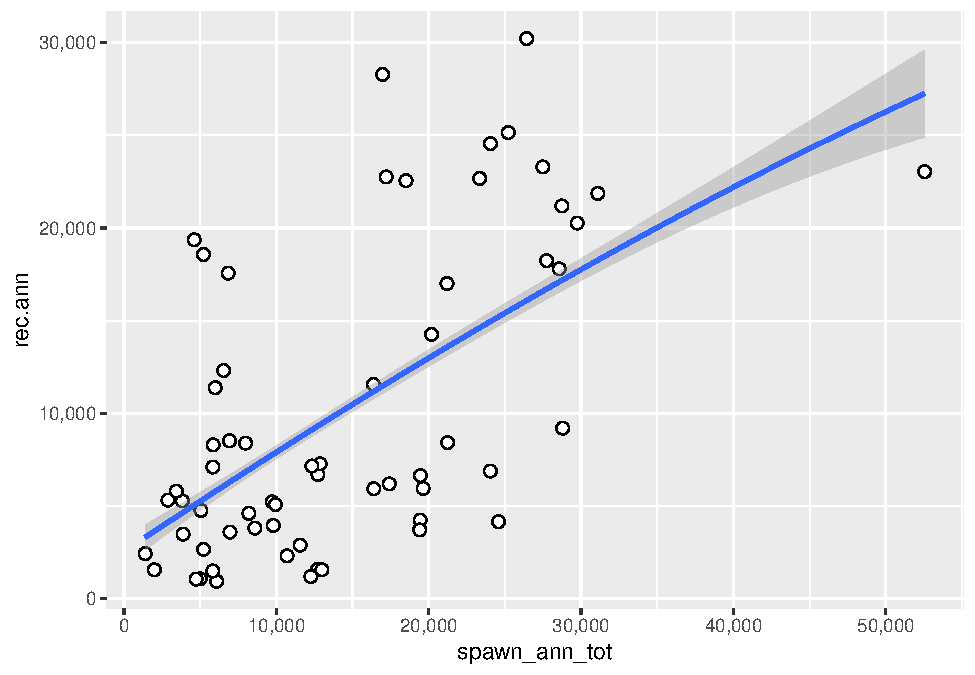
\includegraphics{0_EDM_Vis_Raw_files/figure-latex/unnamed-chunk-4-1.pdf}

\hypertarget{takeaways}{%
\subsubsection{Takeaways}\label{takeaways}}

\hypertarget{total-recruitment-summed-across-all-mpgs-follows-well-known-env-regimes}{%
\paragraph{- Total recruitment (summed across all MPGs) follows well
known env
regimes}\label{total-recruitment-summed-across-all-mpgs-follows-well-known-env-regimes}}

\hypertarget{exhibits-rough-downward-trend}{%
\paragraph{- Exhibits rough downward
trend}\label{exhibits-rough-downward-trend}}

\hypertarget{salmon-recruitment-by-mpg}{%
\subsubsection{Salmon Recruitment by
MPG}\label{salmon-recruitment-by-mpg}}

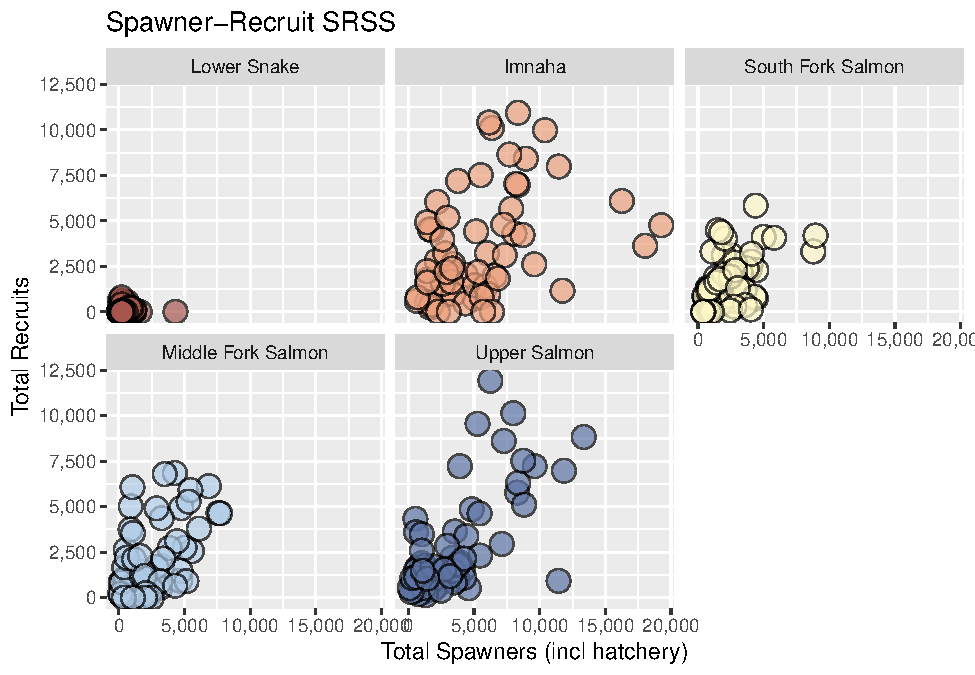
\includegraphics{0_EDM_Vis_Raw_files/figure-latex/unnamed-chunk-5-1.pdf}

\hypertarget{mpgs-share-common-highlow-years-eg-1998-1999-but-of-different-magnitudes}{%
\paragraph{- MPGs share common high/low years (eg 1998-1999) but of
different
magnitudes}\label{mpgs-share-common-highlow-years-eg-1998-1999-but-of-different-magnitudes}}

\hypertarget{but-longer-term-trends-vary-among-mpgs-eg-imnaha-vs-all-salmon-1960-1970}{%
\paragraph{- But longer term trends vary among MPGS (eg Imnaha vs All
Salmon
1960-1970)}\label{but-longer-term-trends-vary-among-mpgs-eg-imnaha-vs-all-salmon-1960-1970}}

\hypertarget{salmon-recruitment-colored-by-mpg}{%
\subsubsection{Salmon recruitment colored by
MPG}\label{salmon-recruitment-colored-by-mpg}}

\includegraphics{0_EDM_Vis_Raw_files/figure-latex/unnamed-chunk-6-1.pdf}

\hypertarget{all-mpgs-declining-overall}{%
\paragraph{- All MPGs declining
overall}\label{all-mpgs-declining-overall}}

\hypertarget{imnaha-and-upper-salmon-historical-strongholds}{%
\paragraph{- Imnaha and Upper Salmon historical
strongholds}\label{imnaha-and-upper-salmon-historical-strongholds}}

\hypertarget{increased-synchronydecreased-portfolio-of-variability-in-given-year}{%
\paragraph{- Increased synchrony/decreased portfolio of variability in
given year
(!)}\label{increased-synchronydecreased-portfolio-of-variability-in-given-year}}

\hypertarget{total-recruitment-and-individual-age-cohorts}{%
\subsubsection{Total Recruitment and individual age
cohorts}\label{total-recruitment-and-individual-age-cohorts}}

\includegraphics{0_EDM_Vis_Raw_files/figure-latex/unnamed-chunk-7-1.pdf}

\hypertarget{year-old-returners-a-declining-proportion-even-esp-in-the-good-year-of-the-mid-aughts}{%
\paragraph{- 5 year old returners a declining proportion even, esp in
the good year of the
mid-aughts}\label{year-old-returners-a-declining-proportion-even-esp-in-the-good-year-of-the-mid-aughts}}

\hypertarget{total-recruitment-and-individual-age-cohorts-by-mpg}{%
\subsubsection{Total Recruitment and individual age cohorts by
MPG}\label{total-recruitment-and-individual-age-cohorts-by-mpg}}

\includegraphics{0_EDM_Vis_Raw_files/figure-latex/unnamed-chunk-8-1.pdf}

\hypertarget{pattern-of-fewe-age-5-not-driven-by-any-one-mpg-but-fairly-robust-pattern}{%
\paragraph{- Pattern of fewe age 5 not driven by any one MPG but fairly
robust
pattern}\label{pattern-of-fewe-age-5-not-driven-by-any-one-mpg-but-fairly-robust-pattern}}

\hypertarget{normalized-recruitment-for-every-stock-in-each-mpg}{%
\subsubsection{Normalized recruitment for every stock in each
MPG}\label{normalized-recruitment-for-every-stock-in-each-mpg}}

\includegraphics{0_EDM_Vis_Raw_files/figure-latex/unnamed-chunk-9-1.pdf}

\hypertarget{stocks-within-mpgs-largely-covary-with-exception-of-north-fork-in-upper-salmon}{%
\paragraph{- Stocks within MPG's largely covary (with exception of North
Fork(!) in Upper
Salmon)}\label{stocks-within-mpgs-largely-covary-with-exception-of-north-fork-in-upper-salmon}}

\hypertarget{plot-total-returns-against-aligned-predictors-facet-by-predictor}{%
\subsubsection{Plot total returns against aligned predictors; facet by
predictor}\label{plot-total-returns-against-aligned-predictors-facet-by-predictor}}

\includegraphics{0_EDM_Vis_Raw_files/figure-latex/unnamed-chunk-10-1.pdf}

\hypertarget{lots-to-unpack-here-first-note-that-salmon-numbers-are-mean-of-normalized-stocks-except-for-in-the-harvest-panel-where-it-is-total-recruitment}{%
\subparagraph{Lots to unpack here, first note that salmon numbers are
mean of normalized stocks (except for in the harvest panel, where it is
Total
Recruitment}\label{lots-to-unpack-here-first-note-that-salmon-numbers-are-mean-of-normalized-stocks-except-for-in-the-harvest-panel-where-it-is-total-recruitment}}

\hypertarget{csl-at-total-population-scale-does-not-seem-to-be-driving-declines}{%
\paragraph{- CSL at total population scale does not seem to be driving
declines}\label{csl-at-total-population-scale-does-not-seem-to-be-driving-declines}}

\hypertarget{closely-correlated-with-pdo-but-total-population-bufffered-against-early-events}{%
\paragraph{- Closely correlated with PDO but total population bufffered
against early
events?}\label{closely-correlated-with-pdo-but-total-population-bufffered-against-early-events}}

\hypertarget{hatchery-releases-coincide-with-major-declines-consistent-with-replacement-hypothesis}{%
\paragraph{- Hatchery releases coincide with major declines consistent
with replacement
hypothesis}\label{hatchery-releases-coincide-with-major-declines-consistent-with-replacement-hypothesis}}

\hypertarget{proportion-harvested-has-tracked-population-incredibly-well-until-recently}{%
\paragraph{- Proportion harvested has tracked population incredibly well
\ldots{} until
recently(!)}\label{proportion-harvested-has-tracked-population-incredibly-well-until-recently}}

\hypertarget{zoom-into-csl-to-see-any-stronger-individual-mpg-correlations}{%
\subsubsection{Zoom into CSL to see any stronger individual MPG
correlations}\label{zoom-into-csl-to-see-any-stronger-individual-mpg-correlations}}

\includegraphics{0_EDM_Vis_Raw_files/figure-latex/unnamed-chunk-11-1.pdf}

\hypertarget{nope}{%
\paragraph{- Nope}\label{nope}}

\hypertarget{zoom-into-harvest-to-look-at-individual-mpg-correlations}{%
\subsubsection{Zoom into harvest to look at individual MPG
correlations}\label{zoom-into-harvest-to-look-at-individual-mpg-correlations}}

\includegraphics{0_EDM_Vis_Raw_files/figure-latex/unnamed-chunk-12-1.pdf}

\hypertarget{seems-that-managers-are-unreasonably-good-at-matching-f-to-abundance-even-at-the-mpg-level-fishy}{%
\paragraph{- Seems that managers are unreasonably good at matching F to
abundance, even at the MPG-level \ldots{}
fishy}\label{seems-that-managers-are-unreasonably-good-at-matching-f-to-abundance-even-at-the-mpg-level-fishy}}

\hypertarget{need-to-dig-up-meta-data-on-harvest-proportion}{%
\paragraph{- Need to dig up meta data on harvest
proportion}\label{need-to-dig-up-meta-data-on-harvest-proportion}}

\hypertarget{now-look-at-covariance-among-predictors}{%
\subsection{Now, look at covariance among
predictors}\label{now-look-at-covariance-among-predictors}}

\includegraphics{0_EDM_Vis_Raw_files/figure-latex/unnamed-chunk-13-1.pdf}

\begin{verbatim}
## NULL
\end{verbatim}

\hypertarget{a-little-hard-to-see-maybe-use-corrplot-for-colors}{%
\paragraph{- A little hard to see, maybe use corrplot for
colors}\label{a-little-hard-to-see-maybe-use-corrplot-for-colors}}

\hypertarget{correlation-heatmap-of-selected-variables}{%
\subsubsection{Correlation heatmap of selected
variables}\label{correlation-heatmap-of-selected-variables}}

\includegraphics{0_EDM_Vis_Raw_files/figure-latex/unnamed-chunk-14-1.pdf}

\hypertarget{strong-positive-correlations-year-x-csl-hatcheries-x-csl-hatcheries-x-srkw}{%
\paragraph{- Strong positive correlations: Year X CSL, Hatcheries X CSL,
Hatcheries X SRKW
(!)}\label{strong-positive-correlations-year-x-csl-hatcheries-x-csl-hatcheries-x-srkw}}

\hypertarget{strong-negative-correlation-pdo-x-csl-pdo-x-recruits}{%
\paragraph{- Strong negative correlation: PDO X CSL, PDO X
Recruits}\label{strong-negative-correlation-pdo-x-csl-pdo-x-recruits}}

\hypertarget{weak-but-notable-recruits-are-positively-linked-to-csl-but-negative-to-srkw}{%
\paragraph{- Weak but notable: Recruits are positively linked to CSL but
negative to
SRKW}\label{weak-but-notable-recruits-are-positively-linked-to-csl-but-negative-to-srkw}}

\hypertarget{time-to-follow-up-simple-correlations-with-some-ccm-results}{%
\subsubsection{Time to follow up simple correlations with some CCM
results
\ldots{}}\label{time-to-follow-up-simple-correlations-with-some-ccm-results}}


\end{document}
